\documentclass{article}
\usepackage[UTF8]{ctex}                     % 支持中文显示
\usepackage{CJKutf8}
\usepackage{amsmath}
\usepackage{listings}
\usepackage{color} %red, green, blue, yellow, cyan, magenta, black, white
\usepackage{xcolor}
\usepackage{incgraph}
\definecolor{mygreen}{RGB}{28,172,0} % color values Red, Green, Blue
\definecolor{mylilas}{RGB}{170,55,241}
\lstset{language=Matlab,%
    %basicstyle=\color{red},
    breaklines=true,%
    morekeywords={imread},
    keywordstyle=\color{blue},%
    morekeywords=[2]{1}, keywordstyle=[2]{\color{black}},
    identifierstyle=\color{black},%
    stringstyle=\color{mylilas},
    commentstyle=\color{mygreen},%
    showstringspaces=false,%without this there will be a symbol in the places where there is a space
    numbers=left,%
    numberstyle={\color{black!40}},% size of the numbers
    numbersep=9pt, % this defines how far the numbers are from the text
    emph=[1]{for,end,break},emphstyle=[1]\color{red}, %some words to emphasise
    %emph=[2]{word1,word2}, emphstyle=[2]{style},
    escapeinside=``
}
\begin{document}
    \title{Function to Output Mathematics Function Image}
    \author{郭炳成}
    \author{Bingcheng Guo}
    \date{\today}
    \maketitle

    图像的边缘,角点,拐点都可以称之为图像的特征点,Laplacian算子利用求图像的二阶微分极值点来获得图像的边缘,二阶微分定义如下:
    \begin{align}
        \Delta = \nabla^2 = \frac{\partial ^2}{\partial x^2} + \frac{\partial ^2}{\partial y^2}\nonumber
    \end{align}

    但是由于laplacian算子对噪声敏感,因此我们首先利用二维高斯核函数对图像进行模糊去噪,然后求二阶微分极值点来获得图像中边缘位置,得


    \begin{align}
        I'(x,y) = g(x,y)* I(x,y)=\iint_D g(x-u,y-u)I(u,v)dudv\nonumber
    \end{align}
   

    \begin{align}
        \Delta \lvert I'(x,y) \lvert = \Delta\lvert g(x,y)*I(x,y)\lvert=
        \frac{\partial^2\iint_D g(x-u,y-v) I(u,v)dudv}{\partial x^2}\nonumber\\ +\frac{\partial^2\iint_D g(x-u,y-v) I(u,v)dudv}{\partial y^2}\nonumber
    \end{align}

    \begin{align}
        \Delta\lvert I'(x,y)\lvert = \iint_D \frac{\partial^2 g(x-u,y-v)}{\partial x^2}I(u,v)dudv\nonumber\\+
        \iint_D \frac{\partial^2 g(x-u,y-v)}{\partial y^2} I(u,v)dudv\nonumber
    \end{align}

    根据卷积结合律得,
    
    \begin{align}
        \Delta\lvert I'(x,y)\lvert = (\frac{\partial^2 g(x,y)}{\partial x^2}+\frac{\partial^2 g(x,y)}{\partial y^2})*I(x,y)
    \end{align}

    由(1)式可知,对图像进行高斯核函数卷积再求二阶微分等价于对高斯核函数先求二阶微分核后再用该核与图像进行卷积。我们定义LoG算子为二阶微分后得高斯核函数

    \begin{align}
        LoG = \Delta\lvert g(x,y)\lvert=\frac{\partial^2 g(x,y)}{\partial x^2}+\frac{\partial^2 g(x,y)}{\partial y^2}\\
        =\frac{\partial^2(\frac{1}{2\pi\sigma^2} e^{-\frac{x^2+y^2}{2\sigma^2}})}{\partial x^2}+\frac{\partial^2(\frac{1}{2\pi\sigma^2} e^{-\frac{x^2+y^2}{2\sigma^2}})}{\partial y^2}\nonumber\\
        =(\frac{x^2}{\sigma^4}-\frac{1}{\sigma^2})\frac{1}{2\pi\sigma^2} e^{-\frac{x^2+y^2}{2\sigma^2}}+(\frac{y^2}{\sigma^4}-\frac{1}{\sigma^2})\frac{1}{2\pi\sigma^2} e^{-\frac{x^2+y^2}{2\sigma^2}}\nonumber\\
        =(\frac{x^2+y^2}{\sigma^4}-\frac{2}{\sigma^2}) \frac{1}{2\pi\sigma^2} e^{-\frac{x^2+y^2}{2\sigma^2}}
    \end{align}

    我们知道归一化二维高斯核
    
    \begin{align}
        g(x,y) = \frac{1}{2\pi\sigma^2} e^{-\frac{x^2+y^2}{2\sigma^2}}\nonumber
    \end{align}

    该函数对$\sigma$进行求导得

    \begin{align}
        \frac{\partial g(x,y)}{\partial\sigma} = \frac{\partial (\frac{1}{2\pi\sigma^2}e^{-\frac{x^2+y^2}{2\sigma^2}})}{\partial\sigma}\nonumber\\
        =\frac{1}{2\pi\sigma^2} e ^{-\frac{x^2+y^2}{2\sigma^2}} \frac{x^2+y^2}{\sigma^3}+\frac{-2}{2\pi\sigma^3} e ^{-\frac{x^2+y^2}{2\sigma^2}}\nonumber\\
        =\frac{1}{2\pi\sigma^2} e^{-\frac{x^2+y^2}{2\sigma^2}}(\frac{x^2+y^2}{\sigma^3}-\frac{2}{\sigma})
    \end{align}

    观察(3)式与(4)式,我们发现其在结果上只相差一个常熟$\sigma$即,

    \begin{align}
        \sigma LoG = \frac{\partial g}{\partial \sigma}
    \end{align}

    首先利用两点做一条直线,然后在直线上任意选取10个点,在图像上另外随机取5个点作为outlier。
    
    效果如下(每次的运行都是随机的点,但是保证同一测试用的点都是相同的):
    \begin{figure}
        \centering
        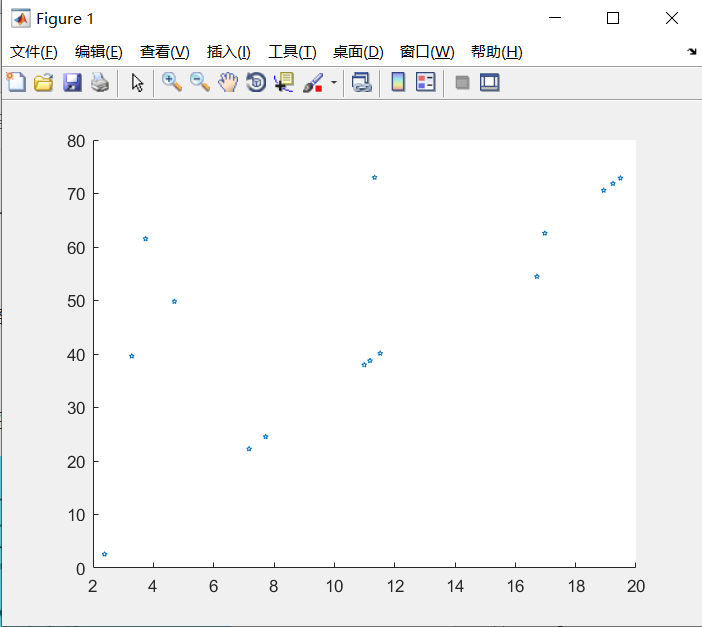
\includegraphics[width=0.7\linewidth]{img/1.png}
        \caption{随机取点}
        \label{}
    \end{figure}

    代码如下:
    \begin{lstlisting}
        a = [2,1];
        b = [20,75];
        x = zeros(1,15);
        y = zeros(1,15);
        for i = 1:10 
            t = rand;
            p = t*a+(1-t)*b;
            x(1,i) = p(1);
            y(1,i) = p(2);
        end

        for i = 11:15
            t = rand;
            s = rand;
            x(i) = t*18+2;
            y(i) = s*74+1;
        end


        scatter(x,y,10,'p','*');%绘制散点图
    \end{lstlisting}

    最小二乘法:
    一系列的点,靠近直线,(假设斜率可求,不是垂直)那么满足条件:
    $y=kx+b$,选取一系列点$(x_i,y_i)$,满足下面的方程:

    \begin{align}
        \begin{bmatrix}
            x_1 & 1\\
            x_2 & 2\\
            \dots\\
            x_n & 1
        \end{bmatrix}
        \begin{bmatrix}
            k\\
            b
        \end{bmatrix}
        =
        \begin{bmatrix}
            y_1\\
            y_2\\
            \dots\\
            y_n
        \end{bmatrix}
    \end{align}
    
    我们规定如下:

    \begin{align}
        X=
        \begin{bmatrix}
            x_1 & 1\\
            x_2 & 2\\
            \dots\\
            x_n & 1
        \end{bmatrix}\nonumber\\
        \beta=
        \begin{bmatrix}
            k\\
            b
        \end{bmatrix}\nonumber\\
        Y=
        \begin{bmatrix}
            y_1\\
            y_2\\
            \dots\\
            y_n
        \end{bmatrix}\nonumber
    \end{align}

    上面(6)式左乘$X^T$,再左乘$(X^T X)^{-1}$,得:

    \begin{align}
        \widehat{\beta}=(X^T X)^{-1}X^T Y
    \end{align}

    拟合得直线得斜率和截距就可以计算出来,matlab代码实现如下:

    \begin{lstlisting}
        a = [2,1];
        b = [20,75];
        x = zeros(1,30);
        y = zeros(1,30);
        for i = 1:25 
            t = rand;
            p = t*a+(1-t)*b;
            x(1,i) = p(1);
            y(1,i) = p(2);
        end                 %得到a,b两点确定得直线

        for i = 26:30
            t = rand;
            s = rand;
            x(i) = t*18+2;
            y(i) = s*74+1;
        end             %加入outlier

        z = ones(1,30);
        x = [x;z];
        ref = (x*x')\x*y';  %计算预测值

        t = [0,10,20];
        s = t*ref(1)+ref(2);    %拟合得直线

        plot(t,s,'-');
        hold on
        plot(x(1,:),y,'*');  %待拟合的各个点
    \end{lstlisting}
    
    效果如图2:
    \begin{figure}
        \centering
        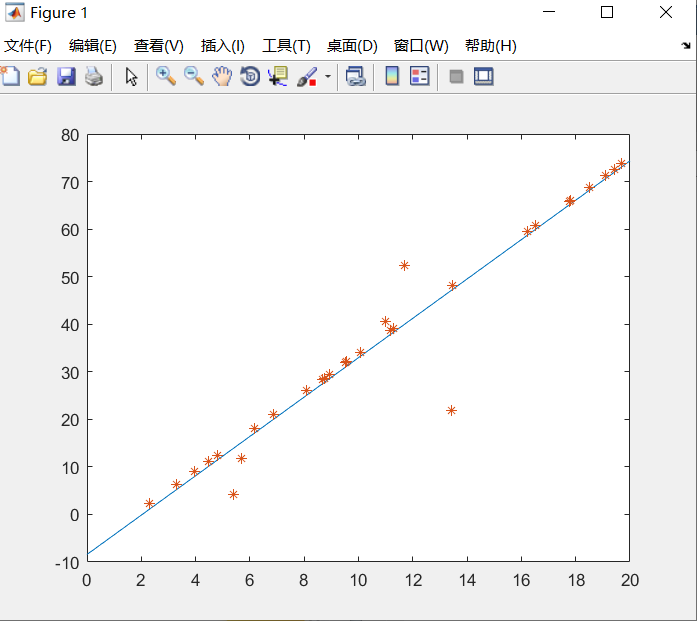
\includegraphics[width=0.7\linewidth]{img/2.png}
        \caption{随机取点}
        \label{}
    \end{figure}

    RANSAC算法就是随机和假设,用抽取得部分样本模拟直线,取几组
    样本中最好的结果,或者过程中已经产生了达到拟合要求的结果就不再继续计算了

    霍夫变换,英文名称Hough Transform,作用是用来检测图像中的直线或者圆等几何图形的。

      一条直线的表示方法有好多种,最常见的是  y=mx+b 的形式。 假设有一幅图像,经过滤
      波,边缘检测等操作,变成了下面这张图的形状,怎么把这张图片中的直线提取出来。基本
      的思考流程是:如果直线 y=mx+b 在图片中,那么图片中,必需有N多点在直线上(像素点
      代入表达式成立),只要有这条直线上的两个点,就能确定这条直线。

      设置两个坐标系,左边的坐标系表示的是(x,y)值,右边的坐标系表达的是(m,b)的值,即直
      线的参数值。那么一个(x,y)点在右边对应的就是是一条线,左边坐标系的一条直线就是右边
      坐标系中的一个点。这样,右边左边系中的交点表示有多个点经过(m,b)确定的直线。但是,
      该方法存在一个问题(m,b)的取值范围太大。

      为了解决(m,n)取值范围过大的问题,在直线的表示方面用 $xcos\theta+ysin\theta=p$ 的规范式代替
      一般表达式,参数空间变成$(\theta,p)$,$0=<\theta<=2\pi$。这样图像空间中的一个像素点在参数空间中
      就是一条曲线(三角函数曲线)。

      Hough Line算法表述如下:

        1、初始化$(\theta,p)$空间,$N(\theta,p)=0$   ($N(\theta,p)$表示在该参数表示的直线上的像素点的个数)

        2、对于每一个像素点(x,y),在参数空间中找出令 $xcos\theta+ysin\theta=p $的$(\theta,p)$坐标,$N(\theta,p)+=1$

        3、统计所有$N(\theta,p)$的大小,取出$N(\theta,p)>threasold$的参数  (threadsold是预设的阈值)

\end{document}